\section{Problems with existing DAGs}
\subsection{Network synchronization}
When a node accepts a request to attach a transaction and attaches the transaction to the local StreamNet, it broadcasts the changes made to its own neighboring machine. When the neighboring machine receives the update, it will follow the basic principles of attaching StreamNet. This update is attached to its own StreamNet and this update is further broadcast. If this update cannot be accepted by a large number of neighboring machines, the probability of being accepted by the entire network is greatly reduced. There are several problems in this:
\begin{itemize}
	\item Issues with offline updates. Offline updates are recognized in StreamNet, but when they are re-online, it will broadcast all local updates, but their local updates will only be accepted in the entire network and will not be partially accepted [4].
	\item How to recognize that a locally confirmed transaction is a transaction accepted by the whole network. How to express it on the wallet is a relatively big problem. In Bitcoin, there is no honest chain and dishonest chain. It is mainly realized by the cost of lying, that is, the POW of exponential growth, wanting to revert the transaction, or constructing the wrong chain. The price is very high. For a wallet, the time to verify a chain is the complexity of polynomial. In this way, we must believe that the data of a certain node in the whole network can be done. Although there are POWs in the current DAG, the complexity of constructing StreamNet itself is polynomial, so for the lying node, it can use a large computing power to construct a wrong StreamNet to mislead the transaction wallet.
	\item Existing DAGs are currently unable to guarantee strong consistency in the network environment [5].
\end{itemize}

\begin{figure}[H]
	\centering
	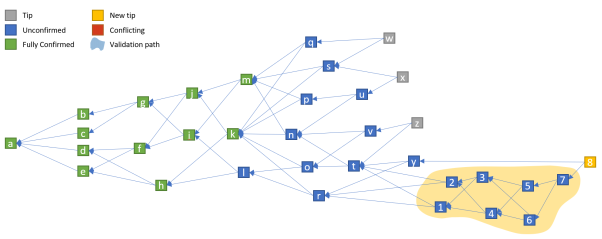
\includegraphics[width=3.0in]{figures/screenshot013.png}
	\caption{Example of offline update [4]}
	\label{simulationfigure}
\end{figure}

\begin{figure}[H]
	\centering
	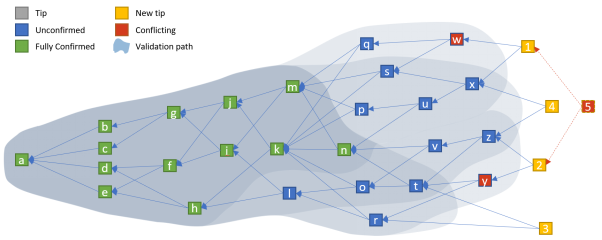
\includegraphics[width=3.0in]{figures/screenshot014.png}
	\caption{Example of double flower problem}
	\label{simulationfigure}
\end{figure}

\subsection{double flower problem}
The double flower problem refers to the problem that the same token is used multiple times, which can be represented by the example in Figure 9, where the two transactions of w and y are double flower transactions, and the transaction 5 is the one that finds that this is a double flower transaction. Transaction. In the transaction consensus, it is obviously impossible to use the 100\% tip confirmation, because there will always be new transactions coming in to break the 100\% confirmation fact. This is called propagation delay [4]. If a random walk algorithm is used, given a confidence level (say 95\%), one of the transactions will naturally receive more transaction approvals in the natural state (without being subjected to a power attack), thus giving it confidence. The degree reaches a state sufficient to be confirmed. For example, as shown in Figure 10, w receives more confirmations in the future, and slowly y is isolated to lose the possibility of being confirmed. But when the fraudster's power is strong enough, it can issue enough transactions to approve w after a transaction is confirmed, then in this case, the previously confirmed transaction will in turn be marginalized. To achieve the purpose of double-flowering, such an attack is a replay attack, and it is necessary to accumulate 34\% of the computing power of the whole network to achieve the goal [6]. However, considering the low number of transactions in the entire network in the early stage [7], 34\% of the power attack is actually not difficult. In order to solve such problems, the transaction confirmed by the coordinator is absolutely valid, so regardless of the computing power of the follow-on attacker. Powerful, can not beat the coordinator's one-vote veto [1]. \\ 
\indent Therefore, the double flower problem is essentially a computing power problem, and it is also the essential problem of the existing DAG system. The introduction of the coordinator is a centralized solution, and in the future, as more and more devices join the StreamNet network, the role of the coordinator It will become unnecessary, and how to remove it to turn DAG into a decentralized network is a challenge [8].

\begin{figure}[H]
	\centering
	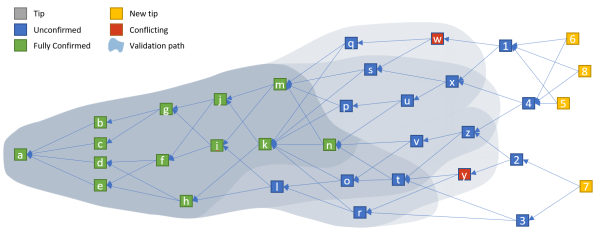
\includegraphics[width=3.0in]{figures/screenshot015.png}
	\caption{Randomly solve the problem of double-flowering}
	\label{simulationfigure}
\end{figure}

\subsection{transaction confirmation speed problem}

\begin{figure}[H]
	\centering
	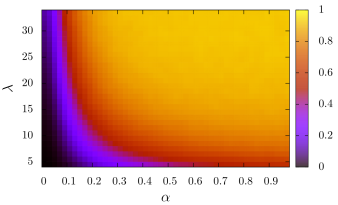
\includegraphics[width=3.0in]{figures/screenshot016.png}
	\caption{The probability of a transaction being permanently stuck (failed), which is random, is the transaction rate [9]}
	\label{simulationfigure}
\end{figure}

The speed at which the transaction is confirmed and the likelihood that the transaction will be finalized depends on two factors, the first is the transaction rate $\lambda$, and the second is the randomness $\alpha$. From Figure 16, it can be seen that the probability of increasing the success of the transaction is mainly to increase the transaction. The rate reduces randomness, and in Figure 17, a more intuitive expression of the effect of $\alpha$ can be seen, under the same conditions, the higher the unconfirmed transaction becomes more. However, because the transaction rate in the whole network is relatively slow, there are not many active nodes, and some optimization methods have been proposed. For example, the method of coordinator mentioned above and the method of Reattach, rebroadcast [10], etc. It can be attributed to the method of human intervention.

\subsection{Encryption Algorithm Vulnerabilities}
Because the current DAG encryption algorithm is based on Trytes, and the encryption algorithm is invented by itself, the method pointed out in [11] can find the hash collision in a few minutes using ordinary computers. The attacker can use this vulnerability to fake other users. Signature, fundamentally disintegrating the security of IOTA.

\subsection{ replay attack}
Replay attacks In addition to the use of power to attack in the double-flower problem, two attack modes are mentioned in the white paper, the first one is a side chain attack and the other is a double-sided chain attack [12]. 

\begin{figure}[H]
	\centering
	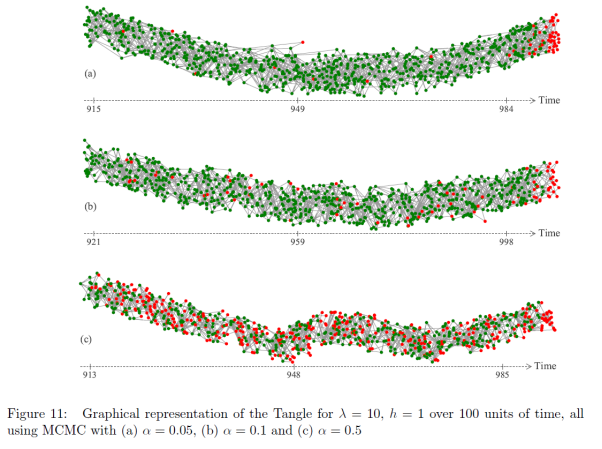
\includegraphics[width=3.0in]{figures/screenshot017.png}
	\caption{a more intuitive expression of the role}
	\label{simulationfigure}
\end{figure}
